\documentclass{beamer} % [aspectratio=169]
\usetheme{ucl}
\setbeamercolor{banner}{bg=darkred}
\setbeamersize{description width=2em}
\setbeamertemplate{navigation symbols}{\vspace{-2ex}} 

\usepackage[T1]{fontenc} % Turn £ into $
\usepackage{minted}
\usemintedstyle{emacs}

\usepackage{fancyvrb}
\usepackage{xcolor}
\usepackage{url}

\usepackage{natbib}
\usepackage{bibentry}
\usepackage{url}

\newenvironment{variableblock}[3]{%
  \setbeamercolor{block body}{#2}
  \setbeamercolor{block title}{#3}
  \begin{block}{#1}}{\end{block}}

\newcommand\emc[1]{\textcolor{midred}{\textbf{#1}}}

\AtBeginSection[]{
  \begin{frame}
  \vfill
  \centering
  \begin{beamercolorbox}[sep=8pt,center,shadow=true,rounded=true]{title}
    \usebeamerfont{title}\insertsectionhead\par%
  \end{beamercolorbox}
  \vfill
  \end{frame}
}

\author{Prof.\ Mark Handley \\ University College London, UK\\
\small{Based on slides from George Danezis}}
\title{Basics of Computer Programming \\ \& Software Engineering (part 2)}
\subtitle{ENGF0002: Design and Professional Skills }
% \institute{}
\date{Term 1, 2019}

\begin{document}
\nobibliography*

\frame{
\titlepage
}

\section{Pebble in the Pond}

\begin{frame}
  \frametitle{Lessons Learned?}

  \begin{itemize}
  \item What worked well?
  \item What didn't work?
  \end{itemize}
\end{frame}  

\begin{frame}
  \frametitle{My observations}
  \begin{itemize}
  \item EEE won.  Why?
  \item Where was the pebble dropped?
  \item Who was in charge?
  \item Was the problem well specified?
  \end{itemize}
\end{frame}

\section{Algorithm of the Week}


\begin{frame}
\frametitle{Euclid's algorithm for computing the GCD. (I)} 

Euclid of Alexandria (300 BC) was interested in properties of integer and rational numbers. 

\vspace{5mm}
Finding the \emc{greatest common denominator} (GCD) allowed them to simplify fractions:

\vspace{5mm}
Eg.\ $\frac{390253}{228769} = \frac{29 \cdot 13457}{17 \cdot 13457} = \frac{29}{17}$ since $GCD(390253, 228769) = 13457$.

\vspace{5mm}
But how to compute the GCD function without resorting to factoring the numbers (which turns out to be a hard problem for large numbers)?

\end{frame}

\begin{frame}
\frametitle{Euclid's algorithm for computing the GCD. (II)} 

\begin{block}{Euclid's algorithm for computing the GCD (in prose)}
\begin{itemize}
\item Consider the two integers for which you want to find the GCD.
\item Take the smaller one, and subtract it from the larger one. 
\item Replace the larger one with this result, and keep the smaller one, as your two new numbers. 
\item Repeat until the two numbers are equal. 
\item Once they are, the resulting (equal) numbers are the GCD.  
\end{itemize}
\end{block}

Let's build a Python program where we execute the concrete steps of the algorithm for the sample numbers 42 and 30.

\end{frame}

\begin{frame}
\frametitle{Why Euclid's algorithm works? (I)}

Consider the positive integers $a$ and $b$:
\begin{align}
a &= \alpha \cdot gcd(a,b), \\
b &= \beta \cdot gcd(a,b),
\end{align}
where $gcd(\alpha, \beta) = 1.$

Without loss of generality, consider $a > b$. After a single step:
\begin{align}
a' &= a - b \\ 
    &= (\alpha - \beta) \cdot gcd(a,b).
\end{align}

Note that $a'$ is always strictly positive.

\end{frame}

\begin{frame}
\frametitle{Why Euclid's algorithm works? (II)}

We can show that $gcd(a', b) = gcd(a,b)$.

Proof by contradiction: 

\begin{itemize}
\item We know that gcd(a,b) is a factor of both a' and b. 
\item So if $gcd(a', b) > gcd(a,b)$ it must be that:
$gcd(\alpha - \beta, \beta) = c > 1$. 
\item Thus we can rewrite $\beta = r \cdot c$ and $\alpha - \beta = r' \cdot c \Leftrightarrow \alpha = (r' + r) \cdot c $. 
\item However that means that $\alpha$ and $\beta$ are both divisible by $c > 1$. \\ Which contradicts $gcd(\alpha, \beta) = 1$.
\end{itemize}

Thus by repeatedly applying the steps of the algorithm we keep the gcd in each step constant while reducing the size of $a$ and $b$. Until they are equal to the gcd.

\end{frame}



\begin{frame}

\frametitle{Calculations following Euclid's algorithm for GCD.} 


	\inputminted[
		xleftmargin=1.4em,
		%frame=lines,
		%framesep=2mm,
		%baselinestretch=1.2,
		bgcolor=stone,
		fontsize=\footnotesize,
		linenos
	]{python}{src/interactive_euclid.py}

\end{frame}

\begin{frame}
\frametitle{Assignments, values \& expressions.}

Let's understand all aspects of the Python code in this example.
\begin{itemize}
\item \emc{Statements} perform an action within the program. In this example all code lines are statements.
\item \emc{Assignments} are statements that assign an expression (right hand side of $=$) to a variable with a number in the program (left hand side of $=$). Eg.\ \mint{python}{a = 42} assigns $42$ to the named variable \texttt{a}.
\item \emc{Expressions} are fragments of code that return a computed quantity.
\item \emc{Values} are expressions that return a constant, eg.\ \texttt{42} and \texttt{30.}
\item More generally \emc{arithmetic expressions} such as \texttt{b - a} perform a computation and return its result. They can be nested arbitrarily.
\end{itemize}

\end{frame}

\begin{frame}
\frametitle{Some Python idioms.}

\begin{itemize}
	\item The order of evaluation of arithmetic expressions follows the \emc{usual precedence rules} of integer arithmetic, eg. \texttt{2+3*4} is computed as \texttt{2+(3*4) = 14}. You may force a different order of evaluation by using parenthesis, eg. \texttt{(2+3)*4 = 20}.
	\item Python allows for multiple \emc{simultaneous assignments}. Eg.\ lines 2--3 could be expressed as:
	\mint{python}{a, b = 42, 30}
	All expressions on the right hand-side are first evaluated before any assignment occurs.
	\item Python allows for \emc{reusing names} in the left-hand side of an assignment as in line 10.
	\mint{python}{b = b - a}
	Only \emc{reuse variable names if they represent the same} high-level concept.

\end{itemize}

\end{frame}

\begin{frame}
\frametitle{Types \& Programming Languages. (I)}

Python is a strongly typed and dynamically typed language. 
\begin{itemize}
\item \emc{Strongly typed}: Every variable, or expression has a \emc{type} associated with it. All expressions in our example program are of type \emc{int} representing integers. Only operations supported by this type can be performed on variables or expressions of that type.
\item \emc{Dynamically typed}: While the program runs the types of objects are tracked, and operations are checked before being applied to ensure they are permitted. 
\end{itemize}

\vspace{5mm}
In contract \emc{statically typed} languages run this check before the program executes. However, to decide \emc{type-safety} before execution they \emc{lose expressiveness} or require \emc{type annotations}.

\end{frame}

\begin{frame}
\frametitle{Types \& Programming Languages. (II)}

\begin{block}{Types and formal methods}
Type systems are the most popular \emc{formal methods} that aid program correctness. They ensure only permissible operations are executed, and eliminate a large number of potential trivial bugs. But are \emc{not a substitute for testing} or further \emc{verification} for correctness.
\end{block}

\end{frame}

\begin{frame}
\frametitle{The Python \texttt{int} integer type} 

The type \emc{int} is primitive, in that the Python language itself knows about it out of the box. It can represent \emc{integers of arbitrary length} (unlike other languages), and supports:
\begin{itemize}
\item The arithmetic operators $+$, $-$, $*$ and $**$ (to the power) return integers.
\item The integer division $//$ and remainder operator $\%$ also return integers.
\item Division $/$, but does not return an integer!
\item The function \texttt{int(x)} returns the integer representation of \texttt{x} (if it exists).
\end{itemize}

\end{frame}

\begin{frame}
\frametitle{Primitive and user-defined types} 

Python supports out-of-the-box a number of types, including integers, complex numbers, real numbers (\texttt{float}), truth values (\texttt{bool}), strings of characters (\texttt{str}), and many data structures.

\vspace{5mm}
A \emc{full list of all supported operations} can be found in the documentation for all primitive types. \emc{Study it} carefully. \url{https://docs.python.org/3/library/stdtypes.html}.


\begin{block}{User-defined types and abstraction}
High-level programming languages allow programmers to define their own types, associated with their own data and permitted operations. This is a key feature that makes programming in such languages expressive---and closer to the intent of the programmer---and free of the need to reflect in very low-level types, minimizing mistakes.
\end{block}

\end{frame}

\begin{frame}[fragile]
\frametitle{Controlling the execution of programs.} 

So far we have used Python as a \emc{glorified calculator}. 

\vspace{2mm}
We had to interpret ourselves the algorithmic commands relating to doing \emc{different operations depending on conditions}, and \emc{repeating operations while a condition holds}.

\vspace{2mm}
\begin{itemize}
	\item \emc{Conditional execution} of commands can be achieved by using the \texttt{if ... then ...} control structure taking the form:
\begin{Verbatim}[fontsize=\scriptsize]
if condition:
    block of statements 1.
else:
    block of statements 2.
\end{Verbatim}

	\item \emc{Repeated execution} while a condition holds may be achieved thorugh the \texttt{while ... } control structure taking the form:
\begin{Verbatim}[fontsize=\scriptsize]
while condition:
    block of statements 1.
\end{Verbatim}

\end{itemize}

\end{frame}

\begin{frame}

\frametitle{Automatic program control for Euclid's algorithm.} 

Refactoring the euclid algorithm to take advantage of \texttt{while} and \texttt{if} control structures.

	\inputminted[
		xleftmargin=1.4em,
		%frame=lines,
		%framesep=2mm,
		%baselinestretch=1.2,
		bgcolor=stone,
		fontsize=\footnotesize,
		%linenos
	]{python}{src/subtraction_euclid.py}

\end{frame}


\begin{frame}

\frametitle{Conditions and the \texttt{bool} type.} 

What is the nature of conditions in Python programs?
\begin{itemize}
\item Conditions are just \emc{expressions}, that return a result of type \emc{bool}.
\item A variable of type \texttt{bool} takes one of two values, \emc{True} or \emc{False}.
\item A number of arithmetic operators return a boolean, including:
  \begin{description}
  \item \texttt{==} for equality
  \item \texttt{<} less than
  \item \texttt{>} greater than
  \item \texttt{!=} not equal, etc.
  \end{description}
%\item The \texttt{bool(x)} function interpets \texttt{x} as a boolean if possible.
\item Booleans may be linked together through `\emc{and}', `\emc{or}' and `\emc{not}'.
\item Those \emc{lazily} evaluate the expressions until its value is determined.
\end{itemize}

\end{frame}


\begin{frame}

\frametitle{Loops, and the \texttt{while} control structure.} 

	\inputminted[
		firstline= 5,
		lastline=9,
		xleftmargin=1.4em,
		frame=lines,
		framesep=2mm,
		%baselinestretch=1.2,
		% bgcolor=stone,
		fontsize=\footnotesize,
		linenos
	]{python}{src/subtraction_euclid.py}

Keep re-executing a block until a condition stops holding.
\begin{itemize}
	\item Upon encountering a \texttt{while} the program \emc{evaluates} the condition.
	\item If the condition is \emc{True} it starts executing the statements in the block.
	\item When the block ends, it \emc{continues} back to the \texttt{while} (line 5).
	\item if \emc{False} it skips the block and \emc{breaks} to line 10.
	\item You can explicitly use \texttt{continue} and \texttt{break} in the program.
\end{itemize}

\end{frame}

\begin{frame}

\frametitle{Conditional execution with the \texttt{if} control structure.} 

	\inputminted[
		firstline= 6,
		lastline=9,
		xleftmargin=1.4em,
		frame=lines,
		framesep=2mm,
		%baselinestretch=1.2,
		% bgcolor=stone,
		fontsize=\footnotesize,
		linenos
	]{python}{src/subtraction_euclid.py}

Execute a block, or another, depending on a condition.
\begin{itemize}
	\item Upon encountering an \texttt{if} the program \emc{evaluates} the condition.
	\item If \emc{True} it executes the first block (line 7).
	\item Else, if \emc{False}, it executes the second block (line 9)
\end{itemize}

\begin{block}{How are blocks defined?}
In Python blocks are defined as a set of statements with the same degree of indentation 
(whitespace). Use 3 or 4 spaces to group blocks together, and do not use any tabs.
\end{block}

\end{frame}

	
\begin{frame}
\frametitle{Euclid as a function.} 

Refactor Euclid's algorithm as a function with two parameters.
	\inputminted[
		xleftmargin=1.4em,
		frame=lines,
		framesep=2mm,
		%baselinestretch=1.2,
		% bgcolor=stone,
		fontsize=\footnotesize,
		linenos
	]{python}{src/subtraction_function_euclid.py}

\end{frame}

\begin{frame}
\frametitle{Re-using code through functions. (I)}

Functions allow us to \emc{define blocks of code}, and \emc{reuse} them without copying them.

	\inputminted[
		firstline=1,
		lastline=1,
		xleftmargin=1.4em,
		frame=lines,
		framesep=2mm,
		%baselinestretch=1.2,
		% bgcolor=stone,
		fontsize=\footnotesize,
		linenos
	]{python}{src/subtraction_function_euclid.py}


\begin{itemize}
	\item Declare a function through the keyword \texttt{def} followed by a \emc{function name}, and a list of \emc{named parameters} in brackets.
	\item The names parameters are \emc{available within the block} (body) of the function, but not outside (\emc{variable scope}).
	\item The \emc{return} statement \emc{exits} the function, and may \emc{return a value}.	
\end{itemize}

	\inputminted[
		firstline=8,
		lastline=8,
		xleftmargin=1.4em,
		frame=lines,
		framesep=2mm,
		%baselinestretch=1.2,
		% bgcolor=stone,
		fontsize=\footnotesize,
		linenos
	]{python}{src/subtraction_function_euclid.py}


\end{frame}


\begin{frame}
\frametitle{Re-using code through functions (II).}

You may call a function, pass to it different parameters, and get the result.

	\inputminted[
		firstline=12,
		lastline=12,
		xleftmargin=1.4em,
		frame=lines,
		framesep=2mm,
		%baselinestretch=1.2,
		% bgcolor=stone,
		fontsize=\footnotesize,
		linenos
	]{python}{src/subtraction_function_euclid.py}


\begin{itemize}
	\item You may \emc{apply} any parameters to a function to \emc{call} it.
	\item \emc{Parameters are expressions} that are evaluated before the function is called.
	\item The function call itself is an expression that results in the \emc{value returned} or \emc{None}. 
\end{itemize}

\vspace{3mm}
Functions are key to supporting \emc{abstraction} in programs.

\end{frame}


\begin{frame}
\frametitle{The `scope' of variables.}

\begin{block}{Why Scope variables?}
Scope ensures that the names of variables from different parts of the program do not clash and 
confuse the programmer, by ensuring a degree of `locality'. 
\end{block}

LEGB Rule defines when variables are available to a block (scope):
\begin{itemize}
\item \emc{L, Local}: Names assigned in any way within a function.
\item \emc{E, Enclosing-function locals}: Name in the local scope of any and all statically enclosing functions, from inner to outer.
\item \emc{G, Global (module)}: Names assigned at the top-level of a module file, or by executing a global statement.
\item \emc{B, Built-in (Python)}: Names in the built-in names module.
\end{itemize}
\end{frame}

\begin{frame}
\frametitle{The Abstraction and DRY principles.}

Benjamin C. Pierce in \emph{Types and Programming Languages} (2002):
\begin{block}{The Abstraction Principle}
Each significant piece of functionality in a program should be implemented in \emc{just one place} in the source code. Where similar functions are carried out by distinct pieces of code, it is \emc{generally beneficial} to combine them into one by \emc{abstracting out} the varying parts.
\end{block}

 Andy Hunt and Dave Thomas in \emph{The Pragmatic Programmer} (1999)
\begin{block}{Don't Repeat Yourself (DRY) Principle}
Every piece of knowledge must have a \emc{single, unambiguous, authoritative representation} within a system.
\end{block}

\end{frame}

\begin{frame}
\frametitle{Euclid as a function and unit test} 

Refactor the Euclid Example with \texttt{ax,bx = 42,30} as a test.
	\inputminted[
		xleftmargin=1.4em,
		frame=lines,
		framesep=2mm,
		%baselinestretch=1.2,
		% bgcolor=stone,
		fontsize=\footnotesize,
		linenos
	]{python}{src/subtraction_function_euclid_test.py}

\end{frame}


\begin{frame}
\frametitle{What makes a good test?}

Brian W. Kernighan and Rob Pike in  \emph{The Practice of programming} (1999), provide some advice:
\begin{itemize}
	\item \emc{Coverage}, make sure all lines, and code paths are tested.
	\item \emc{Compare} different implementations to check refactoring and refinement.
	\item Test for \emc{boundary conditions}, values and special cases.
	\item Identify and test that \emc{pre- and post- conditions} hold.
	\item Identify and check for \emc{conservation properties}.
	\item Check \emc{error} returns and exceptional paths.
\end{itemize}

\vspace{3mm}
Tests cannot check all possible paths of large programs, but \emc{model checkers} can be used to test paths more efficiently.

\end{frame}


\begin{frame}
\frametitle{The `happy path', errors and exceptions.}

Users of your code will use it in \emc{invalid ways}, and \emc{exceptional circumstances} will occur.

\vspace{3mm}
Handling errors and exceptions:
\begin{itemize}
	\item Upon an error code should \emc{fail fast}, and \emc{never fail silently}.
	\item Your \emc{code should handle errors and exceptions} that are the result of external factors.
	\item An external factor is \emc{your future self}, using your own code in an unexpected manner.
	\item Handling exceptional paths must not obscure the intent of your program (the \emc{happy path}).
	\item Use \emc{language facilities} to handle errors and exceptions.
\end{itemize}

\end{frame}

\begin{frame}
\frametitle{Raising an exception upon error.} 

Refactor Euclid to ensure that inputs are positive integers.

	\inputminted[
		highlightlines={3-4},
		firstline=1,
		lastline=10,
		xleftmargin=1.4em,
		frame=lines,
		framesep=2mm,
		% baselinestretch=1.2,
		% bgcolor=stone,
		fontsize=\footnotesize,
		linenos
	]{python}{src/subtraction_function_euclid_exc.py}

The \emc{raise} keyword \emc{interrupts the flow of the program}, and exits the block with an exception immediately.

\end{frame}

\begin{frame}[fragile]
\frametitle{The \texttt{try / except / finally} control structure.}

To \emc{handle an exception raised} by a block of code we use:
\begin{Verbatim}[fontsize=\scriptsize]
try:
    Block that may `raise' exception ExceptionName.
except ExceptionName as VariableName:
    Block that handles the exception.
finally:
    Block that is always executed.
\end{Verbatim}

\begin{itemize}
	\item The program executes the block in \emc{try} until the block ends.
	\item If the block raises an exception, the execution ends, 
	and it is matched to the exception name in the \emc{except} handler.
	\item If the exception matches the block of the exception handler is executed, otherwise the exception is raised further.
	\item In all cases the \emc{finally} block of code is executed.
\end{itemize}

\end{frame}


\begin{frame}
\frametitle{How to test \& handle exceptions.}

A test that ensures the exception handler is activated for invalid input.
	\inputminted[
		firstline=19,
		lastline=29,
		xleftmargin=1.4em,
		frame=lines,
		framesep=2mm,
		%baselinestretch=1.2,
		% bgcolor=stone,
		fontsize=\footnotesize,
		linenos
	]{python}{src/subtraction_function_euclid_exc.py}

Note that multiple, including generic, \emc{except} blocks may be present.
\end{frame}


\begin{frame}
\frametitle{Detect errors at a low level, handle them at a high level.}

The Python raise mechanism interrupts the flow, and bubbles up the exception to outer calling blocks. Why?
\begin{itemize}
\item Errors are often detected \emc{deep within programs}. \\ Eg.\ a file name does not exist when you are about to open it.
\item At such a low-level, it is \emc{not known how to handle} them.
\item Thus error handling happens at a higher level, \\ when \emc{options for recovery} are known.
\item Use the \emc{finally} for local clean-up upon an error.
\item Do not use exceptions as part of the happy path, and vice versa.
\end{itemize}

\vspace{3mm}
Only \emc{handle errors at a level where you know how to recover}, otherwise raise them up further.

\end{frame}


\begin{frame}
\frametitle{The practice of refactoring.}

Programs are living things that \emc{evolve}.
\begin{itemize}
\item Programming is a \emc{dynamic activity}: a program is \emc{re-written and re-tested} many times per minute.
\item Evolving the program to increase its quality is called \emc{refactoring}.
\item \emc{Good design} (abstraction and DRY) \& the existence of \emc{good tests} ensure refactoring does \emc{not introduce new errors} in existing code.
\end{itemize}

\begin{block}{Version Control enables fearless refactoring}
What if refactoring breaks your working program? Tests will detect this, but how can you go back to the working previous version? The solution is to use a version control system, such as \texttt{git}, which we will study later.
\end{block}

\end{frame}

\section{Data Structure of the Week}

\begin{frame}
  \frametitle{Python Lists}
  Often you need to store a bunch of data.  In python, one way to do this is to use a \emc{list}.
	\inputminted[
		xleftmargin=1.4em,
		%frame=lines,
		%framesep=2mm,
		%baselinestretch=1.2,
		bgcolor=stone,
		fontsize=\footnotesize,
		%linenos
	]{python}{src/interactive_lists.py}
  
\end{frame}

\begin{frame}
  \frametitle{Deleting and Inserting in Python Lists}
	\inputminted[
		xleftmargin=1.4em,
		%frame=lines,
		%framesep=2mm,
		%baselinestretch=1.2,
		bgcolor=stone,
		fontsize=\footnotesize,
		%linenos
	]{python}{src/interactive_lists2.py}
  
\end{frame}

\begin{frame}
  \frametitle{Be careful about copying Lists}
	\inputminted[
		xleftmargin=1.4em,
		%frame=lines,
		%framesep=2mm,
		%baselinestretch=1.2,
		bgcolor=stone,
		fontsize=\footnotesize,
		%linenos
	]{python}{src/interactive_lists3.py}
  
\end{frame}

\begin{frame}
  \frametitle{Iterating over Python Lists}
	\inputminted[
		xleftmargin=1.4em,
		%frame=lines,
		%framesep=2mm,
		%baselinestretch=1.2,
		bgcolor=stone,
		fontsize=\footnotesize,
		%linenos
	]{python}{src/interactive_lists4.py}
  
\end{frame}

\section{Week 1 assignments}

\section{Assignment 2: Bomber Game}

\begin{frame}
  \frametitle{Bomber Game}
  \begin{columns}
    \begin{column}{0.5\textwidth}
      \begin{enumerate}
      \item Play the game
      \item Find a bug
      \item Write a bug report
      \item Identify the cause of the bug
      \item Fix the bug
      \item Repeat from 1.
      \end{enumerate}
    \end{column}
    \begin{column}{0.5\textwidth}
      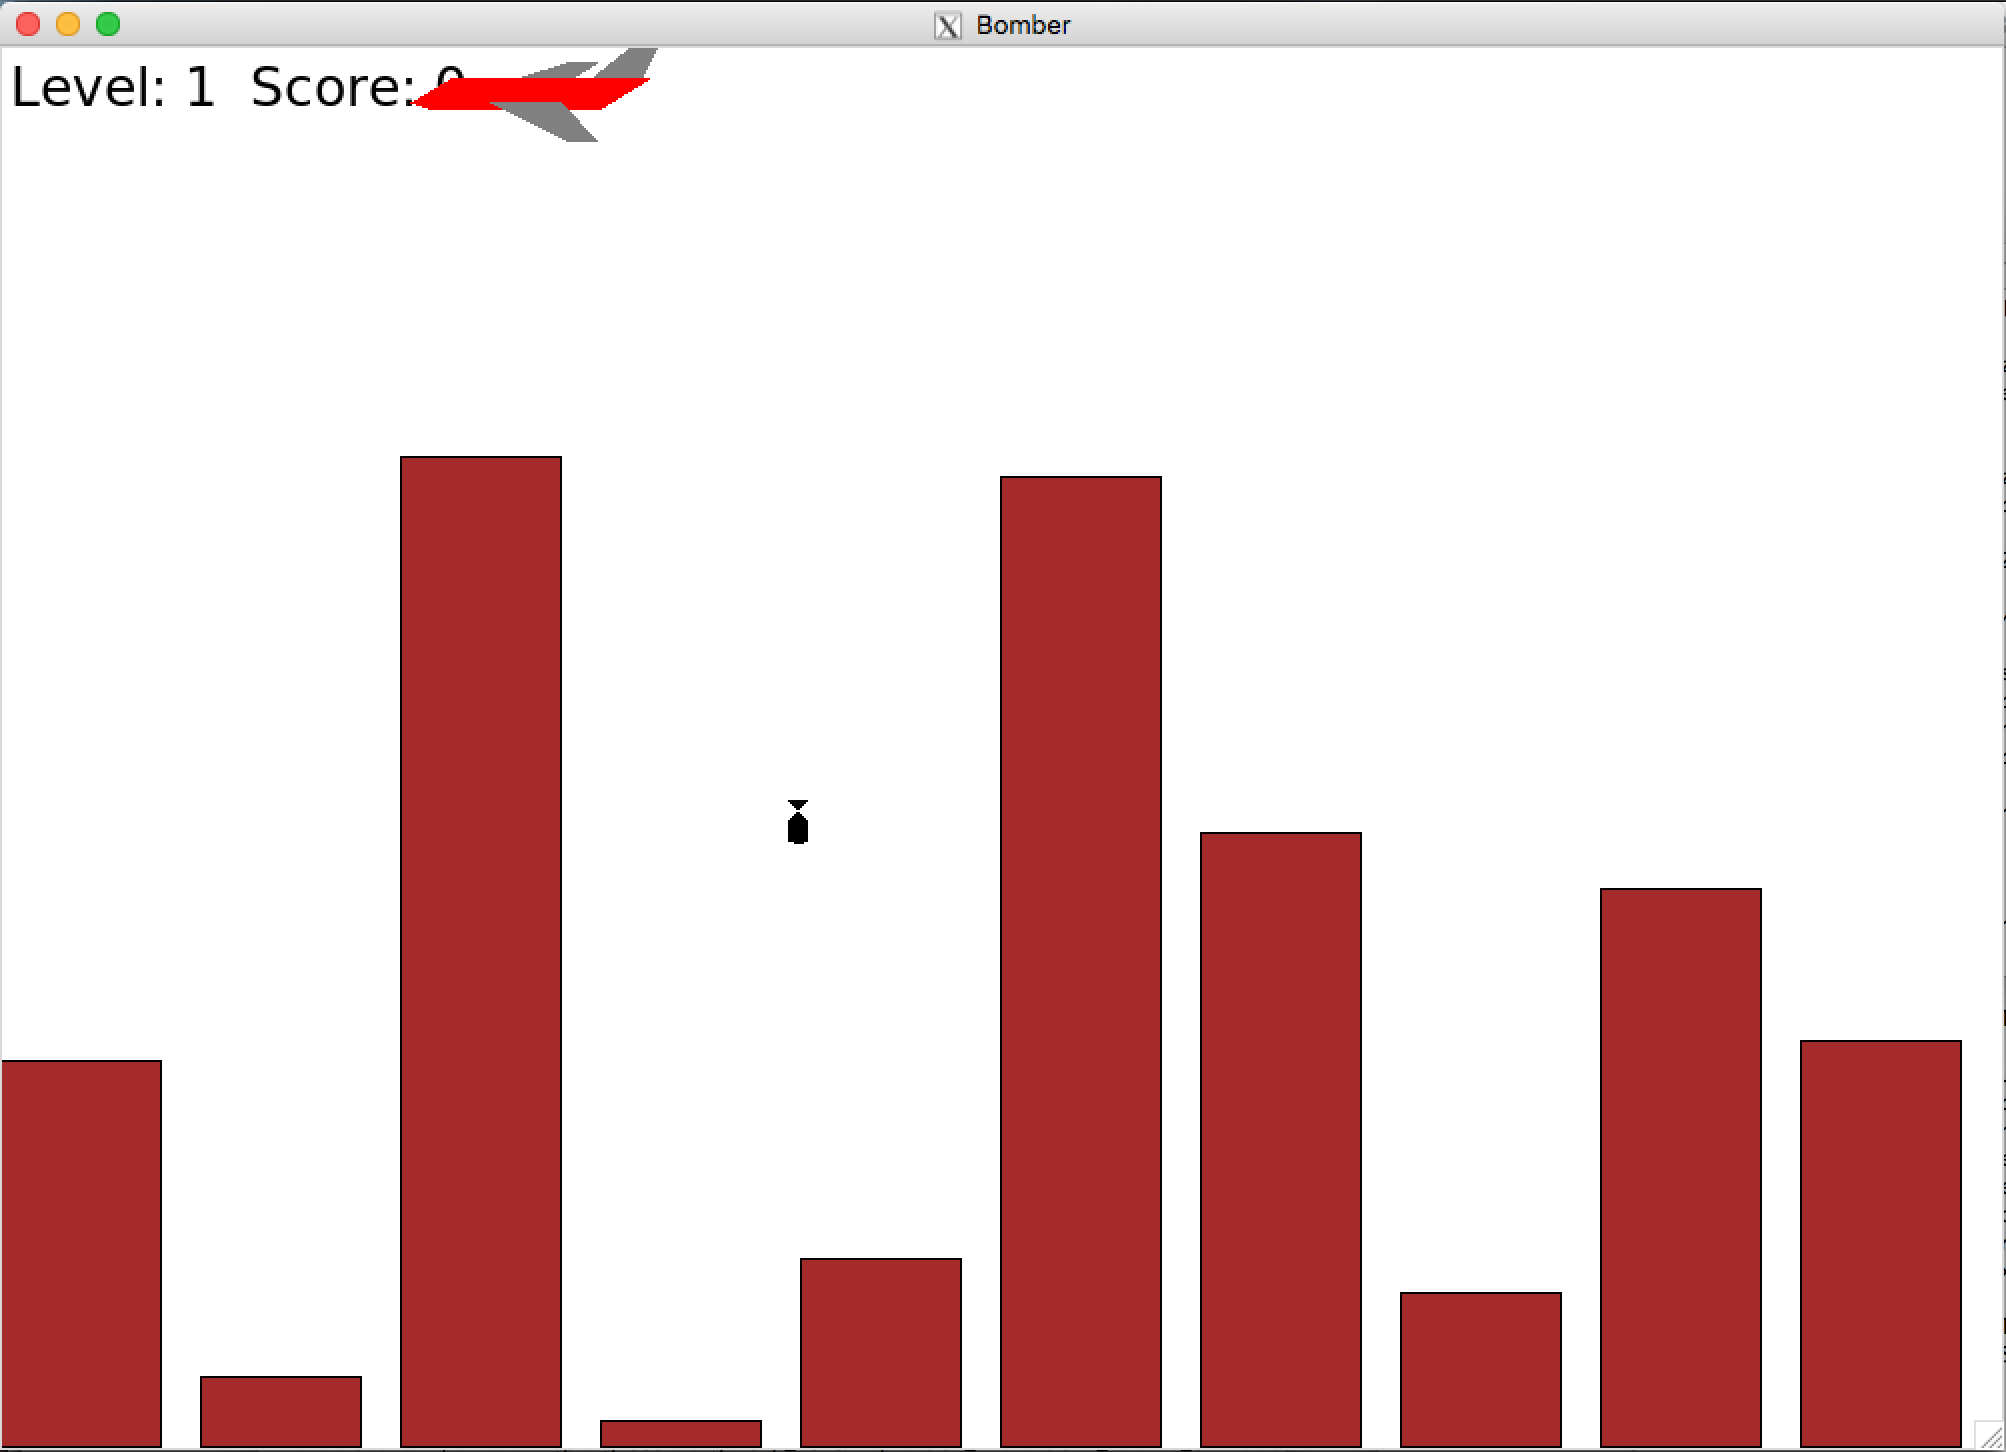
\includegraphics[height=40mm]{img/bomber-example.png}
    \end{column}
  \end{columns}
\end{frame}

\begin{frame}
  \frametitle{Example Bug report}
  \begin{variableblock}{Summary}{bg=stone,fg=black}{bg=black,fg=white}
    Plane flys through building
  \end{variableblock}  
  \begin{variableblock}{What happens}{bg=stone,fg=black}{bg=black,fg=white}
    If the bomb is falling, the plane flys through the buildings without colliding with them.
  \end{variableblock}  
  \begin{variableblock}{What should happen}{bg=stone,fg=black}{bg=black,fg=white}
    Game should terminate when plane hits building, irrespective of whether the bomb is falling.
  \end{variableblock}  
  \begin{variableblock}{How to reproduce}{bg=stone,fg=black}{bg=black,fg=white}
    Drop the bomb just before the plane hits a building.
  \end{variableblock}  
\end{frame}
  
    

\begin{frame}
\frametitle{A strange bug}

	\inputminted[
		xleftmargin=1.4em,
		%frame=lines,
		%framesep=2mm,
		%baselinestretch=1.2,
		bgcolor=stone,
		fontsize=\footnotesize
		%linenos
	]{python}{examples/divide-by-zero.py}

\end{frame}

\begin{frame}
  \begin{variableblock}{Bug report}{bg=stone,fg=black}{bg=black,fg=white}
\tt From:     Sammartino, Matteo <m.sammartino@ucl.ac.uk>\\
To:       m.handley@cs.ucl.ac.uk\\
Subject:  Re: games on Windows\\
Date:     Thursday, October 04, 2018 10:27 AM\\

Hi Mark,\\

I got a division by 0 on line 338:\\

speed = 0.0166/elapsed\\

Matteo
\end{variableblock}  

\end{frame}

\begin{frame}
\frametitle{Bug fixed}

	\inputminted[
		xleftmargin=1.4em,
		%frame=lines,
		%framesep=2mm,
		%baselinestretch=1.2,
		bgcolor=stone,
		fontsize=\footnotesize
		%linenos
	]{python}{examples/nodivide.py}

\end{frame}

\bibliographystyle{alpha}
\nobibliography{references}

\end{document}
